\subsection{Ship scale models}
\label{sec:ship_scale_models}
The data was collected with two scale models of the wind-powered car carrier (wPCC). The smaller 5m model (see \autoref{fig:5m}) with scale factor 1:41 was used in the laboratory experiments in RISE (https://www.sspa.se/) Maritime Dynamics Laboratory (MDL). The larger 7m geosim model (see \autoref{fig:7m}) with scale factor 1:30 was used in the field data experiments \citep{hillenbrand_development_2021}, conducted in a sheltered sea environment in the Stockholm archipelago. The main particulars of the two models are shown in \autoref{tab:main_particulars}. The two models are almost geometrically similar. The only exceptions are that the rudders of the 7m models are slightly more to the aft (5 cm) and that the propeller geometries are different. The 5m model was also equiped with a stabilizer fin as seen in \autoref{fig:5m} which was not present on the 7m model. The geometries differ above the water line however, where the 7m model has a large positive bow angle.

\begin{table}[!ht]
    \centering
    \caption{Main particulars of the 5m and 7m scale models.}
    \label{tab:main_particulars}
    \pgfplotstabletypeset[col sep=comma,
        columns={Particular,Unit,5m,7m},
        columns/Particular/.style={string type},
        columns/Unit/.style={string type},
        columns/5m/.style={string type},
        columns/7m/.style={string type},
        column type=l,	% specify the align method
        every head row/.style={before row=\hline,after row=\hline},	% style the first row
        every last row/.style={after row=\hline},	% style the last row
    ]{tables/ship_main_particulars.main_particulars.csv"}
\end{table}

\begin{figure}[!ht]
    \includegraphics[width=\textwidth]{figures/5m.jpg}
    \caption{5m model. One of the stabilizer fins can be seen at the bilge around the midship section. It can also be seen that the model was equiped with two fans, to test the sailing performance of the ship. These fans are however not used in this paper.}
    \label{fig:5m}
\end{figure}

\begin{figure}[!ht]
    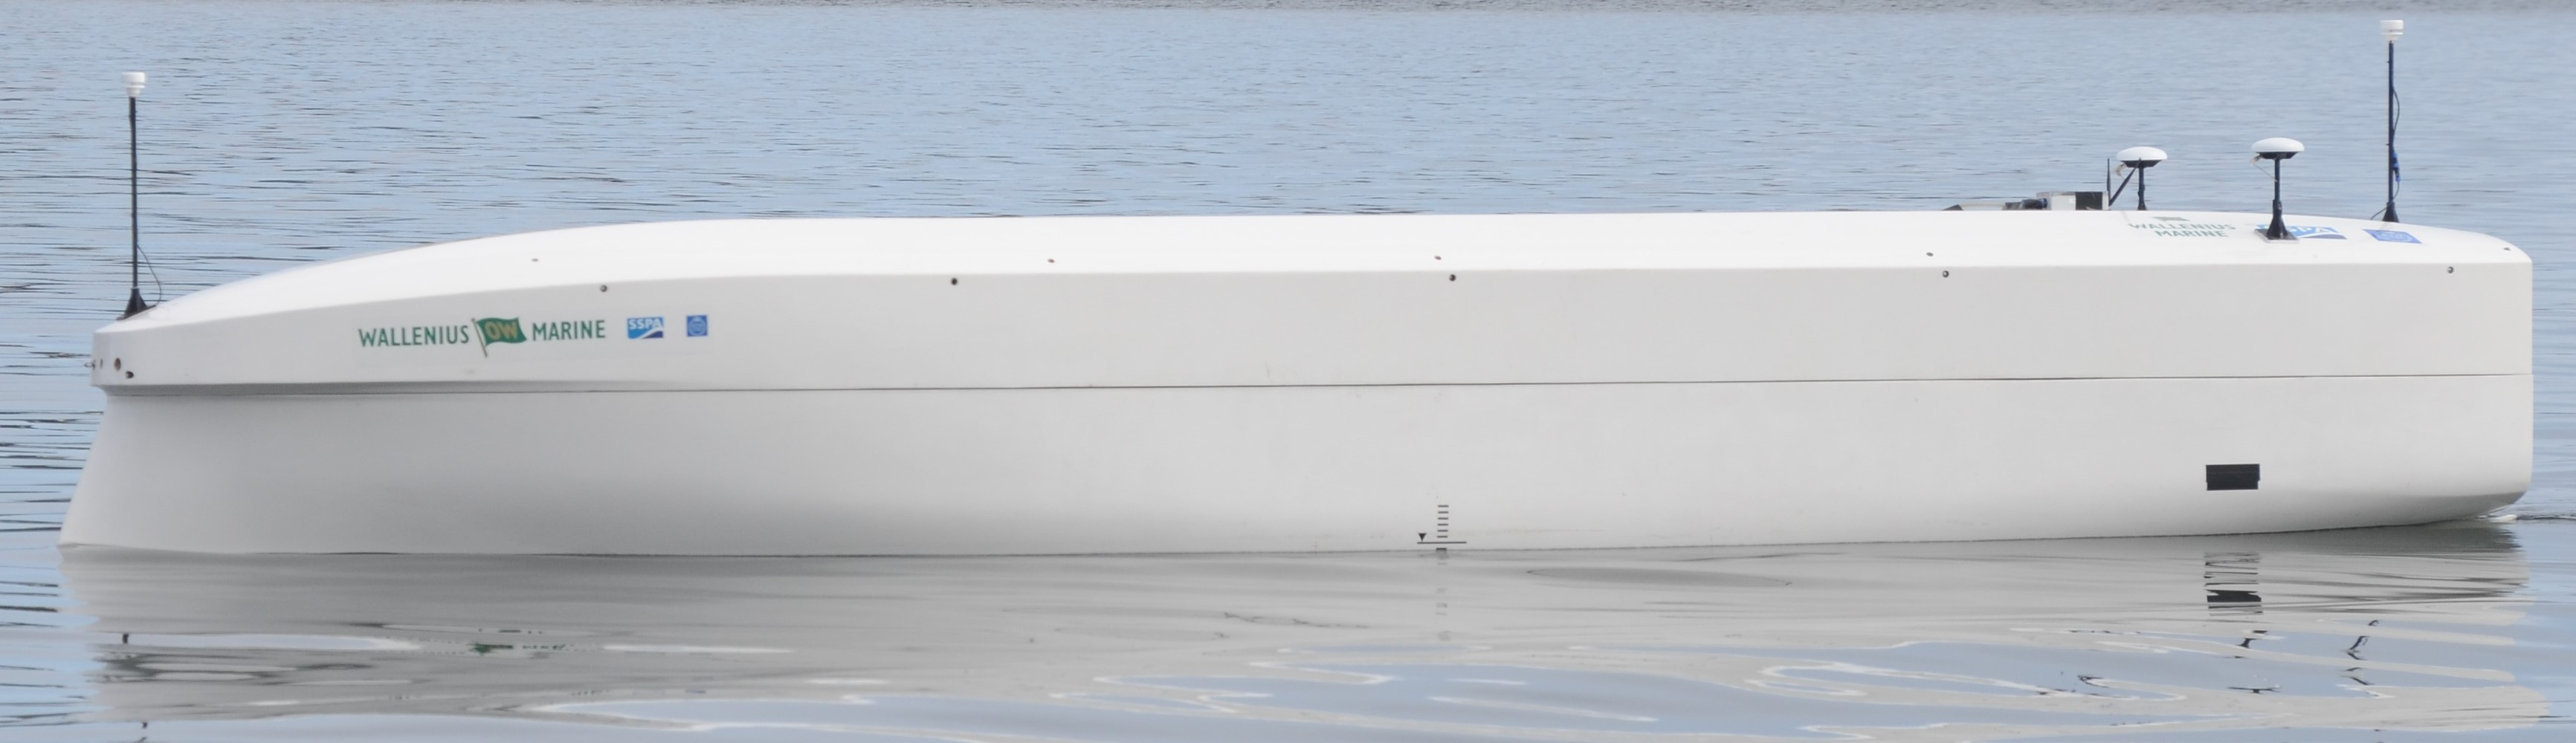
\includegraphics[width=\textwidth]{figures/7m.jpg}
    \caption{7m model. The bow and aft anemometers and the two GPS antennas, in the aft, can be seen ontop of the superstructure.}
    \label{fig:7m}
\end{figure}